\documentclass{article}

% Language setting
% Replace `english' with e.g. `spanish' to change the document language
\usepackage{polski}
\usepackage[utf8]{inputenc}

% Set page size and margins
% Replace `letterpaper' with `a4paper' for UK/EU standard size
\usepackage[letterpaper,top=2cm,bottom=2cm,left=3cm,right=3cm,marginparwidth=1.75cm]{geometry}

% Useful packages
\usepackage{amsmath}
\usepackage{graphicx}
\usepackage[colorlinks=true, allcolors=blue]{hyperref}
\usepackage{multirow}
\usepackage{tabularx}
\usepackage{makecell}

\renewcommand\cellgape{\Gape[4pt]}
\newcolumntype{R}{>{\centering\arraybackslash}X}%
\newcolumntype{C}[1]{>{\centering\let\newline\\\arraybackslash\hspace{0pt}}m{#1}}

\title{Praca inżynierska}
\author{Mikołaj Kuszowski}

\begin{document}
\maketitle

\begin{abstract}
      brak
\end{abstract}

\section{Przegląd popularnych aplikacji do notowania treningów}
      Najwięcej aplikacji do zarządzania treningami na siłowni możemy znaleźć w postaci natywnych aplikacji mobilnych na platformę Android czy iOS. Funkcjonują również aplikacje internetowe, jednak ich popularność jest znikoma w porównaniu z aplikacjami mobilnymi.

      \subsection{FitNotes}
            Jedna z najpopularniejszych aplikacji natywnych na platformę Android. Na czas tworzenia tego dokumentu została pobrana ponad 1 milion razy, a ogólna ocena wynosi 4.8 na 5. Jak podaje oficjalna strona aplikacji jest to "przejrzysta, prosta i wydajna aplikacja do śledzenia treningów" oraz "bezpłatna i bez żadnych reklam" \cite{FitNotesWeb}. Nie udało mi się odnaleźć dokładnej daty premiery aplikacji w Google Play, ale pierwsze wzmianki o tej aplikacji pochodzą z 2013 roku. 
            \subsubsection*{Mechanizm działania}
                  Po zainstalowaniu aplikacji jest ona gotowa do używania. Nie ma możliwości rejestracji i logowania, z tego powodu wszystkie dane o naszym treningu przechowywane są lokalnie na urządzeniu. Po uruchomieniu aplikacji możemy zobaczyć widok główny, w którym znajduje się: widok treningu z aktualnego dnia, nawigacja oraz przyciski dodawania i kopiowania treningu.
            \subsubsection*{Zalety}
                  \begin{itemize}
                        \item Bezpłatny i bez reklam. Aplikacja mimo, że jest darmowa nie wyświetla żadnych reklam dzięki czemu jest bardzo przyjemna w użytkowaniu.
                        \item Prostota obsługi. Na stronie aplikacji twórca w pierwszym zdaniu zwraca uwagę na to, że FitNotes jest łatwy i przejrzysty. Aplikacja spełnia swoją rolę przy czym nie posiada funkcjonalności, które zaburzyły by wygodę użytkowania.
                        \item Skalowalność i elastyczność. Poprzez ten punkt trzeba rozumieć rozszerzalność aplikacji o kolejne ćwiczenia. Po zainstalowaniu aplikacji dostępna jest baza podstawowych ćwiczeń, jednak użytkownik ma możliwość dodania swoich własnych.
                        \item Śledzenie postępów. W aplikacji możemy zweryfikować swój progres na każdym ćwiczeniu poprzez wykres bazujący na wyliczeniach 1RM (rep max). Dzięki temu możemy zweryfikować postęp na przestrzeni miesiąca, roku czy wszystkich treningów.
                        \item Prosty backup. Mimo, że dane znajdują się lokalnie na naszym urządzeniu, istnieje możliwość stworzenia kopii zapasowej i zapisaniu pliku w dowolnym miejscu. Samo wgranie kopii zapasowej również jest bardzo proste. Dzięki temu uszkodzenie urządzenia lub zmiana telefonu nie powoduje straty historii naszego postępu.
                  \end{itemize}
            \subsubsection*{Wady}
                  \begin{itemize}
                        \item Brak połączenia z serwerem. Aplikacja nie jest połączona z żadnym serwerem, w związku z tym wszystkie dane znajdują się na naszym urządzeniu. Tym samym musimy pamiętać o tworzeniu kopii zapasowej i zapisywaniu jej w bezpiecznym miejscu, tak aby nie stracić historii progresu.
                        \item Brak aplikacji na innych platformach. Aplikacja FitNotes została stworzona na platformę Android i nie doczekała się publikacji na żadnym innym systemie. Przez co zmiana telefonu na system przykładowo iOS niestety uniemożliwi kontynuowanie naszej historii progresu.
                  \end{itemize}
      \subsection{Hevy}
            Ta aplikacja również jest bardzo popularna, z Google Play została pobrana ponad milion razy, a użytkownicy Androida oceniają ją na 4.9 na 5 gwiazdek. Hevy jest darmowe, ale ilość funkcjonalności w porównaniu z poprzednią aplikacją jest dużo większa. Główną różnicą jest konieczność założenia konta. Dzięki temu mamy możliwość powrotu do naszych wcześniejszych osiągnięć bez konieczności wgrywania kopii zapasowej. Jednak nasze konto nie służy tylko do przechowywania informacji o treningach. Hevy możemy traktować jako portal społecznościowy zrzeszający osoby trenujące na siłowni. Możemy wstawić swoje zdjęcie profilowe czy wprowadzić pseudonim. Możemy zaobserwować innych użytkowników, żeby śledzić ich progres w treningu. Podobnie inni użytkownicy mogą zaobserwować nas. Jeżeli nie chcemy, aby inni użytkownicy mieli dostęp do naszego profilu, możemy ustawić konto jako prywatne.
            \subsubsection*{Mechanizm działania}
            Po uruchomieniu aplikacji konieczna jest rejestracja lub zalogowanie się do istniejącego konta. Po poprawnym uwierzytelnieniu możemy rozpoczynać korzystanie z aplikacji. Mamy do dyspozycji 3 zakładki:
            \begin{itemize}
                  \item Home (Strona główna)
                  \item Workout (Trening)
                  \item Profile (Profil)
            \end{itemize}
            Na stronie głównej możemy zobaczyć nasze treningi oraz wpisy użytkowników, których śledzimy. W zakładce trening możemy dodać nowy trening lub dodać nową rutynę treningową czyli stworzyć plan treningowy, który będziemy powielać w innych dniach. Możemy również wybrać trening z gotowych planów treningowych udostępnianych przez aplikację. W zakładce profil możemy zmienić ustawienia konta, dodać pomiary ciała, czy zaobserwować innych użytkowników.
            \subsubsection*{Zalety}
            \begin{itemize}
                  \item Posiadanie konta. Dzięki konieczności rejestracji nie musimy martwić się o nasze dane, ponieważ będą synchronizowane i wysyłane do serwera i zapisywane w globalnej bazie danych.
                  \item Bezpłatny i bez reklam. Aplikacja jest darmowa i nie wyświetla reklam, ale istnieje płatna wersja "pro", która udostępnia dodatkowe funkcjonalności. 
                  \item Skalowalność. Aplikacja umożliwia dodawanie kolejnych ćwiczeń z wyborem typu ćwiczenia np. ciężar i powtórzenia, czas, czas i dystans. Umożliwia to odpowiednie skonfigurowanie ćwiczenia ze względu na jednostki zapisu. 
                  \item Śledzenie postępów. Można sprawdzić swój progres, jednak w darmowej wersji tylko na przestrzeni ostatnich 3 miesięcy.
                  \item Dodatkowe funkcjonalności. Aplikacja może stać się portalem społecznościowym, na którym będziemy mogli obserwować bardziej doświadczone osoby z branży fitness.
                  \item Mobilna multiplatformowość. Aplikacja jest dostępna na platformie iOS oraz Android.
            \end{itemize}
            \subsubsection*{Wady}
            \begin{itemize}
                  \item Poziom skomplikowania. Udostępnia wiele funkcjonalności, z których większość osób nigdy nie skorzysta. Przez większą ilość opcji aplikacja staje się mniej przejrzysta i trudniejsza w obsłudze.
                  \item Wersja premium. Mimo, że aplikacja jest darmowa to kilka istotnych funkcjonalności np. weryfikacja progresu z ostatniego roku, jest zablokowana w wersji darmowej.
                  \item Dostępna tylko jako natywna aplikacja mobilna.
            \end{itemize}
      \subsection{Simple Workout Log}
            Jest jedną z pierwszych aplikacji jaką można znaleźć po wpisaniu w wyszukiwarkę internetową frazy "web gym tracker". Aplikacja jest darmowa i bez reklam.
            \subsubsection*{Mechanizm działania}
            Aby móc z niej korzystać najpierw konieczna jest rejestracja. Aplikacja mimo, że wydaje się prosta, wymaga od nas początkowo dużego nakładu pracy. Wynika to z braku początkowej bazy ćwiczeń. Dostępne zakładki to:
            \begin{itemize}
                  \item Exercise (ćwiczenie)
                  \item Category (kategoria)
                  \item Routine (rutyna)
                  \item Tools (ustawienia)
            \end{itemize}
            W zakładce ćwiczenia można wyświetlić dostępne ćwiczenia oraz dodać nowe. Zakładka kategorie jest odpowiedzialna za uporządkowywanie ćwiczeń. Możemy stworzyć kategorię odpowiadającą odpowiedniej grupie mięśniowej i dodać do niej wybrane ćwiczenia. Zakładka rutyna jest podobna do zakładki kategoria, ponieważ możemy stworzyć rutynę i dodać do niej odpowiednie ćwiczenia. Jednak ta zakładka służy głównie do uporządkowywania ćwiczeń ze względu na dzień treningowy. Po wejściu w odpowiednią rutynę możemy zmieniać kolejność ćwiczeń. Można również wykorzystać opcję rozpoczynania rutyny, która będzie wyświetlała szczegóły dodanego ćwiczenia i przechodziła do następnego po zapisaniu notatek. W zakładce ustawienia mamy możliwość dodania informacji o naszej masie ciała.
            \subsubsection*{Zalety}
            \begin{itemize}
                  \item Bezpłatna i bez reklam. Aplikacja jest darmowa, bez reklam i nie posiada zablokowanych opcji dostępnych tylko w wersji premium.
                  \item Posiadanie konta. Wszystkie informacje o naszych treningach zapisywane są na serwerze, dzięki temu nie musimy martwić się o bezpieczeństwo naszych danych na lokalnym urządzeniu.
                  \item Multiplatformowość. Dzięki temu, że aplikacja jest dostępna z poziomu przeglądarki możemy notować treningi z każdego urządzenia, nawet komputera.
                  \item Skalowalność. Aplikacja umożliwia dowolne tworzenie i konfigurowanie ćwiczeń i kategorii.
            \end{itemize}
            \subsubsection*{Wady}
            \begin{itemize}
                  \item Brak wstępnej bazy ćwiczeń. Po rejestracji witają nas puste widoki. Konieczność wpisania wszystkich ćwiczeń wykonywanych na siłowni, nawet tych bardzo popularnych może zniechęcić użytkownika do korzystania z aplikacji.
                  \item Nieintuicyjna. Aplikacja wygląda na prostą, bez dużej ilości funkcjonalności, ale układ aplikacji jest bardzo mylący dla użytkownika. Po uruchomieniu aplikacji nie jest wiadome co powinniśmy najpierw zrobić. Zakładki są nieoczywiste i niepotrzebne z poziomu panelu bocznego.
                  \item Brak podziału ze względu na datę. Standardem w tego typu aplikacjach stało się porządkowanie widoku ze względu na aktualny dzień. Dzięki temu aplikacja jest dużo bardziej przejrzysta i łatwiej odnaleźć się w dużej ilości treningów.
                  \item Brak śledzenia postępów. Aplikacja nie udostępnia żadnych wykresów pokazujących progres na przestrzeni danego okresu.
            \end{itemize}
      \subsection{Lift Book}
            Kolejną aplikacją internetową jest Lift Book. Aplikacja jest darmowa ale istnieje możliwość wpłacenia dobrowolnej wpłaty. Lift Book został stworzony przez osobę, która ćwiczy na siłowni ponad 10 lat i której brakowało prostego narzędzia do notowania treningów z poziomu komputera stacjonarnego jak i z poziomu urządzenia mobilnego.
            \subsubsection*{Mechanizm działania}
                  Aplikacja wymaga rejestracji. Po zalogowaniu się dostępnych jest kilka zakładek:
                  \begin{itemize}
                        \item Home (strona główna)
                        \item Exercises (ćwiczenia)
                        \item History (historia)
                        \item Dashboard (panel)
                  \end{itemize}
                  Na stronie głównej jest możliwość dodania nowego programu. W programie znajdują się rutyny, a w nich lista ćwiczeń. Żeby rozpocząć trening trzeba stworzyć rutynę. W zakładce ćwiczenia można dodać nowe ćwiczenia, które potem można wybrać przy tworzeniu rutyny. Ćwiczenia można dowolnie konfigurować jednak dostępną jednostką jest tylko LBS. W zakładce historia możemy sprawdzić zakończone treningi. Z poziomu widoku o nazwie panel można zobaczyć podsumowanie osiągnięć. Należy dodać, że jest możliwość zaimportowania gotowych planów treningowych. Może to nam zaoszczędzić czas przy dodawaniu ćwiczeń, ale również może być przydatne dla początkujących, którzy nie potrafią ułożyć własnego planu treningowego.
            \subsubsection*{Zalety}
                  \begin{itemize}
                        \item Bezpłatna i bez reklam. Aplikacja została stworzona przez fanatyka siłowni, którą postanowił udostępnić publicznie za darmo. Można jednak wprowadzić dobrowolną wpłatę.
                        \item Posiadanie konta. Możemy zalogować się na dowolnym urządzeniu i korzystać z wcześniejszej konfiguracji.
                        \item Skalowalność i elastyczność. Aplikacja pozwala na stworzenie dowolnego treningu jak i również gotowego szablonu.
                        \item Intuicyjność i prostota obsługi. Aplikacja jest dość intuicyjna i nie jest bardzo rozbudowana co ułatwia jej obsługiwanie.
                        \item Śledzenie postępów. Aplikacja posiada dodatkowy panel, na którym możemy w łatwy sposób zweryfikować nasze postępy i sprawdzić statystyki.
                  \end{itemize}
            \subsubsection*{Wady}
                  \begin{itemize}
                        \item Rozpoczęcie treningu. Trening można rozpocząć tylko z wcześniej stworzonej rutyny. 
                        \item Brak dynamicznej edycji. Nie można modyfikować rutyny np. poprzez zmniejszenie ilości serii czy zmianę ćwiczeń w rozpoczętym treningu. Konieczna byłaby wcześniejsza edycja rutyny, aczkolwiek takie zmiany wymagają większej elastyczności z poziomu treningu.
                        \item Brak bazy ćwiczeń. Istnieje możliwość importu planu treningowego (programu), co implikuje automatyczny import ćwiczeń wykorzystanych w danych rutynach. Jednakże brakuje podstawowych ćwiczeń do wykorzystania bez dodatkowego importu.
                        \item Widok historii. Widok wyświetla chronologicznie posortowane treningi wraz z datą ich wykonania, ale brakuje możliwości ich łatwego wyszukiwania.
                        \item Brak elastyczności. Nie ma możliwości wyboru jednostki masy ciężaru podczas konfiguracji ćwiczenia.
                  \end{itemize}
      \subsection{Porównanie aplikacji do zarządzania treningami pod względem funkcjonalności}
            W tabeli \ref{tab:porownanie_popularnych_aplikacji} porównano wcześniej opisane aplikacje do zarządzania treningami na siłowni. 
            \begin{table}[ht]
                  \renewcommand{\arraystretch}{2}
                  \begin{center}
                        \begin{tabular}{ |C{2,67cm}|C{2,67cm}|C{2,67cm}|C{2,67cm}|C{2,67cm}| }
                              \hline
                                    \multirow{2}{*}{Cechy} 
                                          & \multicolumn{4}{c|}{Aplikacje do zarządzania treningami} \\ \cline{2-5}
                                          & FitNotes & Hevy & Simple Workout Log & Lift Book \\ \hline
                                    Darmowa & Tak & Tak & Tak & Tak \\ \hline
                                    Intuicyjność & Dobra & Średnia & Słaba & Dobra \\ \hline
                                    Baza ćwiczeń & Tak & Tak & Nie & Tak (po imporcie planu treningowego) \\ \hline
                                    Multiplatformowa & Nie & Tylko mobilna & Tak (przeglądarka) & Tak (przeglądarka) \\ \hline
                                    Konieczność rejestracji & Nie & Tak & Tak & Tak \\ \hline
                                    Skalowalna & Tak & Tak & Tak & Tak \\ \hline
                                    Śledzenie postępów & Dobre & Dobre, ale częściowo płatne & Średnie & Dobre \\ \hline
                                    Portal społecznościowy & Nie & Tak & Nie & Nie \\ \hline
                                    Kopiowanie treningów & Tak & Tak & Nie & Nie \\ \hline
                                    Tworzenie planów treningowych & Tak & Tak & Nie & Tak \\ \hline
                                    Gotowe plany treningowe & Nie & Tak & Nie & Tak \\
                              \hline
                        \end{tabular}
                        \caption{Porównanie popularnych aplikacji do zarządzania treningami na siłowni}
                        \label{tab:porownanie_popularnych_aplikacji}
                  \end{center}
            \end{table}
            \subsubsection*{Podobieństwa}
                  \begin{enumerate}
                        \item Darmowa: Wszystkie aplikacje są darmowe i nie wyświetlają żadnych reklam.
                        \item Skalowalność: Aplikacje umożliwiają rozszerzenie bazy ćwiczeń dla danego użytkownika.
                        \item Śledzenie postępów: Każda aplikacja umożliwia w lepszy lub gorszy sposób weryfikacje progresu dla danego ćwiczenia.
                  \end{enumerate}
            \subsubsection*{Różnice}
                  \begin{enumerate}
                        \item Intuicyjność:
                              \begin{enumerate}
                                    \item FitNotes: Aplikacja bardzo prosta do opanowania. Płynnie odkrywamy kolejne funkcjonalności aplikacji w trakcie korzystania z niej. Stworzenie pierwszego treningu wymaga tylko kilku prostych kliknięć, a nawigacja po aplikacji jest bardzo przejrzysta.
                                    \item Hevy: Jest bardziej skomplikowany od FitNotes. Zawiera nieco więcej funkcjonalności związanych z samym notowaniem treningów, ale również zawiera moduł przypominający portal społecznościowy. Przez te funkcjonalności aplikacja może być nieco bardziej przytłaczająca dla nowych użytkowników.
                                    \item Simple Workout Log: Mimo, że aplikacja początkowo wygląda na bardzo prostą to jej działanie nie jest oczywiste. Poza niezrozumiałą nawigacją, konieczne jest stworzenie własnych ćwiczeń co wymaga dużego nakładu pracy. 
                                    \item Lift Book: Dzięki możliwości zaimportowania planów treningowych i ćwiczeń, aplikacja staje się bardzo czytelna i zrozumiała.
                              \end{enumerate}
                        \item Baza ćwiczeń: 
                              \begin{enumerate}
                                    \item FitNotes: Aplikacja zawiera solidną bazę ćwiczeń, która na pewno jest wystarczająca na sam początek.
                                    \item Hevy: Tak samo jak w przypadku aplikacji FitNotes mamy do dyspozycji wystarczającą bazę ćwiczeń.
                                    \item Simple Workout Log: Brak bazy ćwiczeń uniemożliwia płynne korzystanie z aplikacji.
                                    \item Lift Book: Początkowo nie ma żadnej bazy ćwiczeń, jednak jest ona automatycznie wgrywana po zaimportowaniu planu treningowego.
                              \end{enumerate}
                        \item Multiplatformowość: 
                              \begin{enumerate}
                                    \item FitNotes: Aplikacja dostępna tylko w systemie Android.
                                    \item Hevy: Dostępna tylko jako natywna aplikacja mobilna jednak możliwa do pobrania na platformie Android oraz iOS.
                                    \item Simple Workout Log: Dostępna jako aplikacja przeglądarkowa.
                                    \item Lift Book: Podobnie jak Simple Workout Log jest dostępna z poziomu przeglądarki.
                              \end{enumerate}
                        \item Sposób przechowywania danych: 
                              \begin{enumerate}
                                    \item FitNotes: Dane są przechowywane tylko i wyłącznie na urządzeniu lokalnym. Aby przenieść dane na inne urządzenie konieczne jest stworzenie kopii zapasowej.
                                    \item Hevy: Dane są przechowywane na serwerze.
                                    \item Simple Workout Log: Dane są przechowywane na serwerze.
                                    \item Lift Book: Dane są przechowywane na serwerze.
                              \end{enumerate}
                        \item Powielanie treningów: 
                              \begin{enumerate}
                                    \item FitNotes: Umożliwia tworzenie planów treningowych, a także skopiowanie treningu z dowolnego dnia.
                                    \item Hevy: Daje możliwość stworzenia planu treningowego lub wybrania treningu z bazy gotowych planów treningowych. Można również skopiować trening z dowolnego dnia.
                                    \item Simple Workout Log: Nie ma żadnej możliwości powielenia całości treningu. Za każdym razem konieczne jest stworzenie nowego pustego treningu.
                                    \item Lift Book: Można stworzyć plan treningowy i później powielać go oraz można wybrać trening z bazy gotowych planów treningowych.
                              \end{enumerate}
                        \item Dodatkowe funkcjonalności: 
                              Aplikacja Hevy jest najbardziej rozbudowaną aplikacją, a jej główną dodatkową funkcjonalnością jest moduł przypominający portal społecznościowy, na którym można dzielić się zdjęciami i postępami w treningu.
                  \end{enumerate}
            \subsubsection*{Podsumowanie}
                  Jeżeli do planowania treningu i do zapisywania aktualnego progresu wykorzystujemy tylko urządzenie z platformą Android idealnym rozwiązaniem będzie aplikacja FitNotes. Hevy jest rozwiązaniem dla bardziej wymagających użytkowników, którzy od takiej aplikacji oczekują nie tylko możliwości zapisywania postępów, ale również chcą chwalić się swoimi postępami i śledzić postęp innych osób. Aplikacje Simple Workout Log i Lift Book będą idealne dla użytkowników chcących korzystać z aplikacji na każdym urządzeniu, bez konieczności instalowania dodatkowych aplikacji. Simple Workout Log spodoba się użytkownikom poszukujących minimalistycznej aplikacji bez żadnej bazy ćwiczeń czy planów treningowych. Osoby, które cenią intuicyjność połączoną z bazą ćwiczeń czy treningów bardziej docenią aplikację Lift Book.

\section{Specyfikacja nieformalna}
      \subsection{Analiza metodą Human-Centered Design}
            Human Centered Design jest podejściem do projektowania aplikacji skupiające się na człowieku. Uwzględnia użytkowników końcowych na każdym etapie projektowania. Najważniejszym elementem tego podejścia jest zrozumienie czego użytkownik potrzebuje.
      \subsection{Zdefiniowanie problemu}
            W podejściu Human Centered Design jak wspomnieliśmy wcześniej najważniejszym aspektem jest zrozumienie potrzeb użytkownika. Mając to na uwadze sformułowano następujący problem:
            \begin{enumerate}
                  \item Osoby trenujące na siłowni chcą w szybkim tempie zapisywać swoje treningi lub nimi zarządzać.
            \end{enumerate}
            Rozwiązaniem tego problemu będzie:
            \begin{enumerate}
                  \item Zaprojektowanie aplikacji, która w przejrzysty sposób pozwoli notować treningi oraz nimi zarządzać.
            \end{enumerate}
      \subsection{Użytkownicy systemu (Personas)}
            Tak jak wcześniej zostało wspomniane, Human-Centered Design skupia się na użytkowniku końcowym. Dlatego, żeby lepiej zrozumieć potrzeby odbiorcy konieczne będzie stworzenie persony. Persona to realistyczny profil użytkownika końcowego danego produktu lub usługi. Po wstępnej analizie można stwierdzić, że użytkownikiem korzystającym z aplikacji będzie kulturysta, którego profil został przedsawiony w tabeli \ref{tab:profil_uzytkownika_kulturysta}.
            \begin{table}[ht]
                  \renewcommand{\arraystretch}{2}
                  \begin{center}
                        \begin{tabular}{ |C{4,7cm}|C{10cm}|}
                              \hline
                                    Kategoria & Opis \\ \hline
                                    Persona & Kulturysta \\ \hline
                                    Dane demograficzne & \makecell{Wiek: 12+ \\ Płeć: dowolna \\ Stan cywilny: dowolny} \\ \hline
                                    Tło & Osoba ćwicząca na siłowni, posiadająca wiedzę na temat wykonywanych ćwiczeń. \\ \hline
                                    Potrzeby & Aplikacja powinna umożliwić szybkie notowanie treningów pomiędzy wykonywanymi seriami. \\ \hline
                                    Cele & Wybranie dostępnego ćwiczenia i zanotowanie aktualnie wykonywanej serii \\ \hline
                                    Frustracje & Konieczność notowanie treningu w zeszycie co znacznie wydłuża czas spędzony na siłowni \\ \hline
                                    Postrzeganie & Użytkownik będzie musiał wybrać ćwiczenie i zanotować swoje aktualne wyniki \\ \hline
                                    Motywacja & Uproszczenie notowania treningu i ograniczenie czasu tego procesu do minimum \\
                              \hline
                        \end{tabular}
                        \caption{Profil użytkownika kulturysta}
                        \label{tab:profil_uzytkownika_kulturysta}
                  \end{center}
            \end{table}

      \subsection{Historie użytkowników (User stories)}
            Po opisaniu użytkowników systemu, możemy rozpocząć proces opisywania wymagań naszego systemu. Zrobimy to za pomocą tzw. "historyjek użytkowników". Są one tworzone z perspektywy użytkownika końcowego czyli z perspektywy wcześniej stworzonych personas.
            \subsubsection*{Użytkownik kulturysta}
            \begin{enumerate}
                  \item Jako kulturysta chcę móc założyć konto w aplikacji, aby śledzić swoje postępy i planować treningi na każdym urządzeniu.
                  \item Jako kulturysta chcę móc zresetować hasło, aby móc dalej korzystać ze swojego konta jeśli zapomnę hasła.
                  \item Jako kulturysta chcę móc samodzielnie planować trening na dany dzień z listy dostępnych ćwiczeń, aby dopasować trening do swoich potrzeb.
                  \item Jako kulturysta chcę widzieć kalendarz z zaplanowanymi i odbytymi treningami, po to żebym mógł zweryfikować poprzednio odbyty trening lub lepiej organizować czas.
                  \item Jako kulturysta chcę móc skopiować wcześniej wykonany trening, żeby nie musieć układać go od początku i żeby móc weryfikować szczegóły wcześniej wykonanych serii ćwiczeniowych.
                  \item Jako kulturysta chcę wyświetlić listę ćwiczeń zaplanowanych na dzień wybrany z kalendarza, aby wiedzieć jakie ćwiczenia będę wykonywał.
                  \item Jako kulturysta chcę rejestrować wykonane serie i powtórzenia, aby śledzić postępy.
                  \item Jako kulturysta chcę usunąć ćwiczenie z treningu, po to abym mógł wykluczyć ćwiczenie jeżeli nie jest możliwe do wykonania w danym dniu.
                  \item Jako kulturysta chcę móc edytować serię ćwiczeniową, po to abym mógł wprowadzać zmiany względem zaplanowanego lub skopiowanego treningu.
                  \item Jako kulturysta chcę usunąć serię ćwiczeniową, żeby móc wykluczyć serię, która nie została wykonana na danym treningu.
                  \item Jako kulturysta chcę zmieniać kolejność ćwiczeń w zaplanowanym treningu, żeby kolejność ćwiczeń odpowiadała rzeczywistości w przypadku konieczności zmiany aktualnie wykonywanego ćwiczenia.
                  \item Jako kulturysta chcę dodać własne ćwiczenie, żebym mógł zanotować mniej popularne lub autorskie ćwiczenie.
                  \item Jako kulturysta chcę stworzyć plan treningowy, aby powielać go w wybrane dni treningowe.
            \end{enumerate}

      \subsection{Priorytety historii użytkowników}
            Wcześniej zdefiniowane historie użytkowników są używane jako zadania do wykonania w tzw. backlogu projektu. Jednak przed przystąpieniem do ich realizacji ważna jest ich priorytetyzacja. Jest to proces oceny, które historie użytkowników powinny zostać zrealizowane w pierwszej kolejności. W tabeli \ref{tab:priorytety_historii_uzytkownikow} przypisano priorytety do każdej historii użytkowników (mniejsza liczba oznacza wyższy priorytet) wraz z decyzją o jej implementacji.
            \begin{table}[ht]
                  \renewcommand{\arraystretch}{2}
                  \begin{center}
                        \begin{tabular}{ |C{4.8cm}|C{3cm}|C{3cm}|C{3cm}|}
                              \hline
                                    Użytkownik & Historia użytkownika & Priorytet & Implementacja \\ \hline
                                    \multirow{2}{*}{Kulturysta} 
                                          & 1 & 0 & TAK \\ \cline{2-4}
                                          & 2 & 0 & TAK \\ \cline{2-4}
                                          & 3 & 0 & TAK \\ \cline{2-4}
                                          & 4 & 1 & TAK \\ \cline{2-4}
                                          & 5 & 1 & TAK \\ \cline{2-4}
                                          & 6 & 0 & TAK \\ \cline{2-4}
                                          & 7 & 0 & TAK \\ \cline{2-4}
                                          & 8 & 0 & TAK \\ \cline{2-4}
                                          & 9 & 0 & TAK \\ \cline{2-4}
                                          & 10 & 0 & TAK \\ \cline{2-4}
                                          & 11 & 0 & TAK \\ \cline{2-4}
                                          & 12 & 2 & NIE \\ \cline{2-4}
                                          & 13 & 2 & NIE \\
                              \hline
                        \end{tabular}
                        \caption{Priorytety historii użytkowników}
                        \label{tab:priorytety_historii_uzytkownikow}
                  \end{center}
            \end{table}

      \subsection{Makiety ekranów aplikacji}
            W celu wizualnego przedstawienia interfejsu użytkownika przed jego implementacją przygotowano makiety ekranów. Są one kluczowe w projektowaniu aplikacji i weryfikacji funkcjonalności przed rozpoczęciem kodowania, ponieważ pozwala zespołowi zrozumieć, jak dokładnie aplikacja ma działać i wyglądać. Na rysunkach poniżej przedstawiono makiety stworzone za pomocą programu figma, wykorzystujące historie użytkowników zakwalifikowane do wdrożenia.
            \begin{figure}[ht]
                  \centering
                  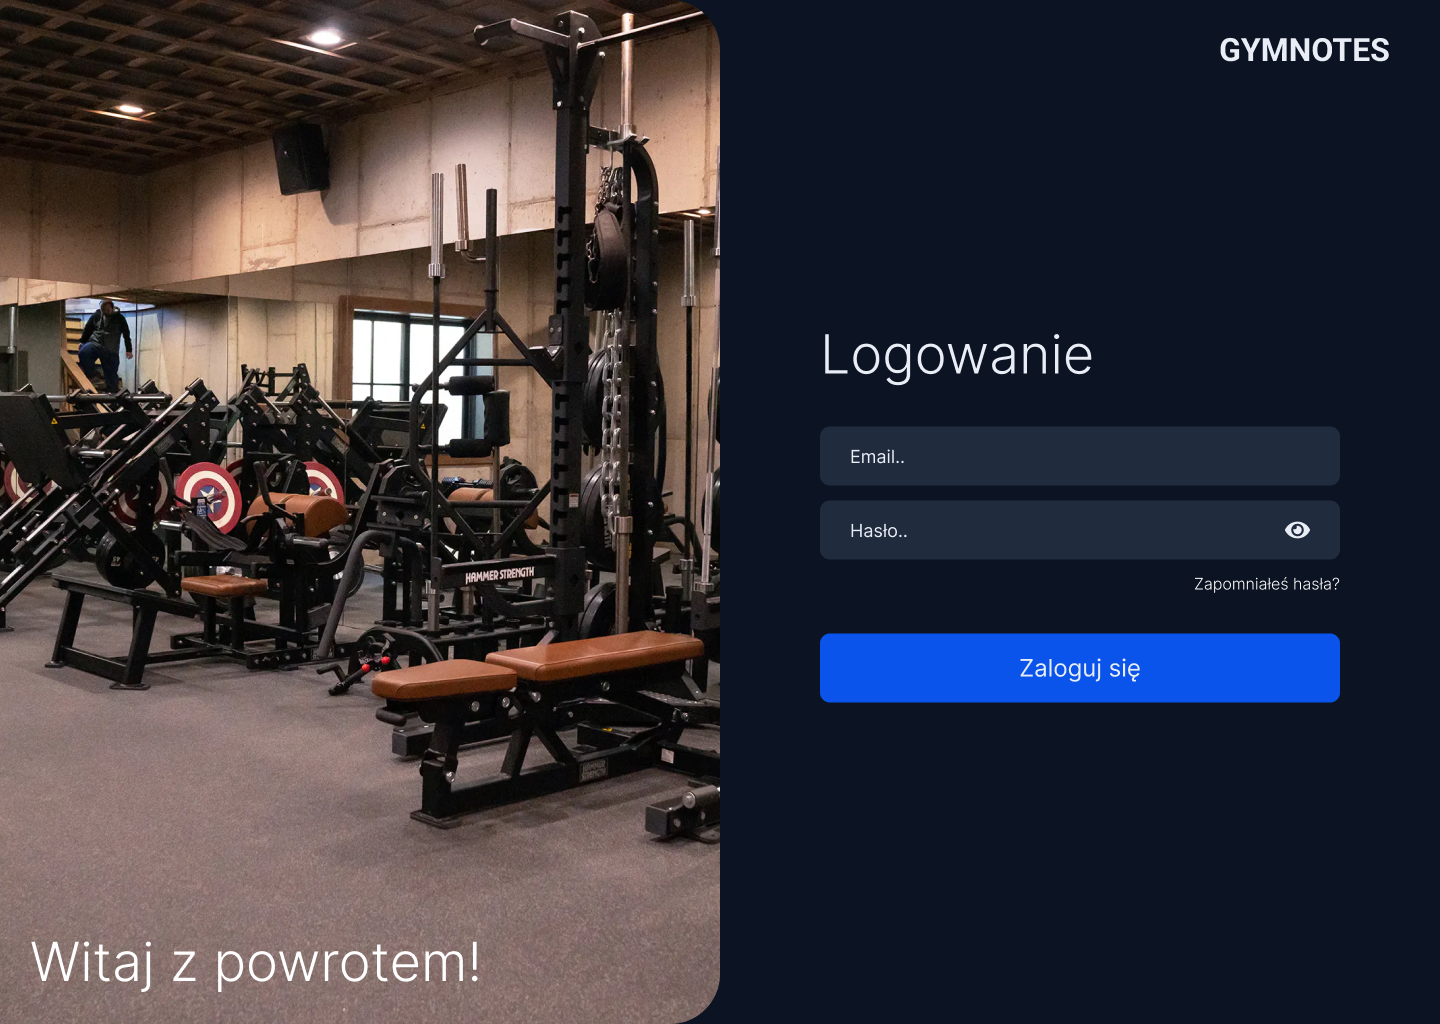
\includegraphics[height=8cm]{Logowanie.png}
                  \caption{Makieta aplikacji; logowanie}
            \end{figure}
            \begin{figure}[ht]
                  \centering
                  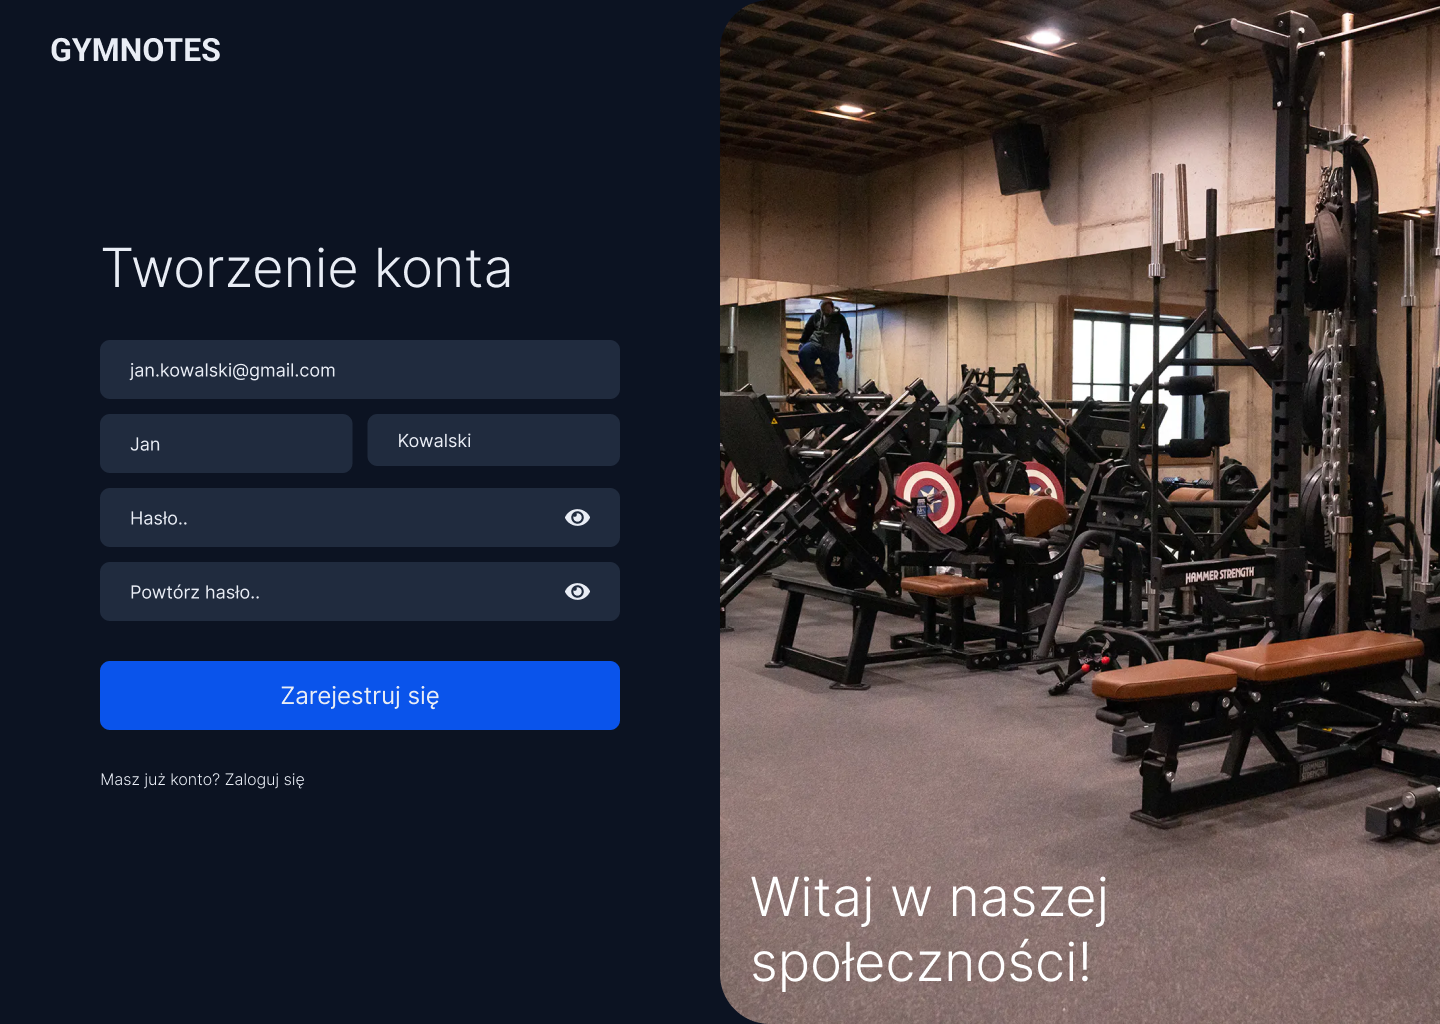
\includegraphics[height=8cm]{Tworzenie konta.png}
                  \caption{Makieta aplikacji; tworzenie konta}
            \end{figure}
            \begin{figure}[ht]
                  \centering
                  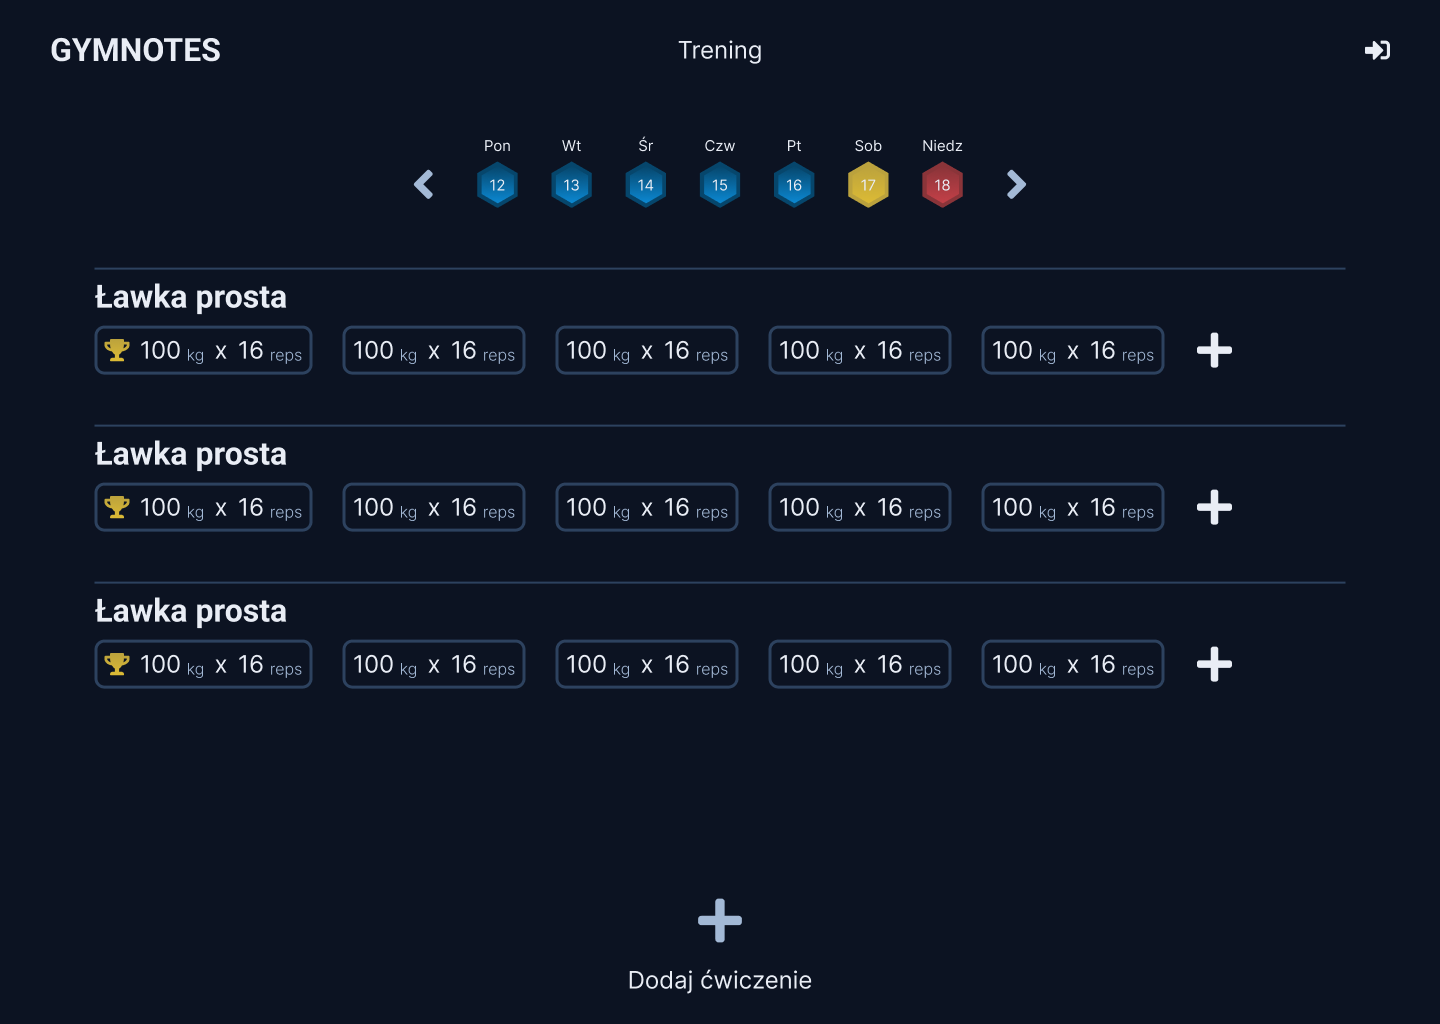
\includegraphics[height=8cm]{Trening.png}
                  \caption{Makieta aplikacji; strona główna z głównymi funkcjonalnościami}
            \end{figure}

      \bibliographystyle{plain}
      \bibliography{refs}
\end{document}